\documentclass[12pt,fleqn]{article}\usepackage{../../common}
\begin{document}
Sonlu Öğeler Metotu (Finite Elements Method -FEM-) - 3

İki boyutta FEM kullanımına gelelim. Diyelim ki alttaki gibi bir problem
yarattım,

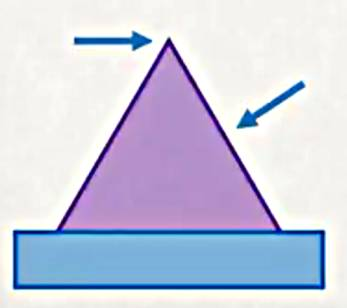
\includegraphics[width=10em]{compscieng_bpp45fem3_01.jpg}

Üçgen şeklinde bir yapı var, onun üzerinde iki noktadan kuvvet uygulanmış, şimdi
bu üçgendeki stres ve gerilmeyi bulmak istiyorum. Bu problemi nasıl çözerdik?
Euler-Bernoulli kiriş denklemini kullanmak zor, şekil ona uygun değil. Zor bir
iş.

Fakat üstteki problemi bir FEM problemine dönüştürürsem işler
kolaylaşabilir. Bir ızgara oluşturabilirim mesela,

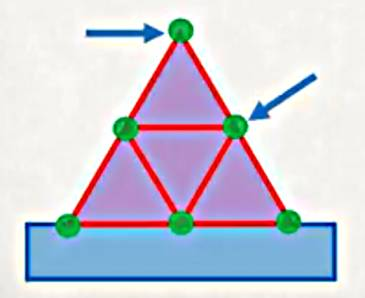
\includegraphics[width=10em]{compscieng_bpp45fem3_02.jpg}

Altı tane düğüm noktası ortaya çıktı, düğümsel yer değişimini hesaplayabiliriz,
ve dikkat edersek düğümlerin üçü altta sabitlenmiş halde. Ama hesapla devam
etmem için o görülen tüm yapının direngenliğini (stiffness) bulmam lazım, bu
derste göreceğimiz ilk konu o ızgaradaki her üçgenin ayrı ayrı direngenliğini
bulabilmek çünkü düğümler üzerindeki kuvvetleri biliyorsam (ki biliyorum)
direngenliği kullanarak çözümde ilerleyebilirim.

Hatırlarsak çubuk ve kirişleri modellerken bir yaklaşıklama fonksiyonu
kullanmıştım, bu fonksiyon yukarı ya da yana doğru bir hareketi, yer değişimini
yaklaşık olarak temsil ediyordu. İki boyutta benzer bir prosedürü kullanacağız,
fakat tek yön yerine iki yönü aynı anda temsil etmemiz gerekecek.

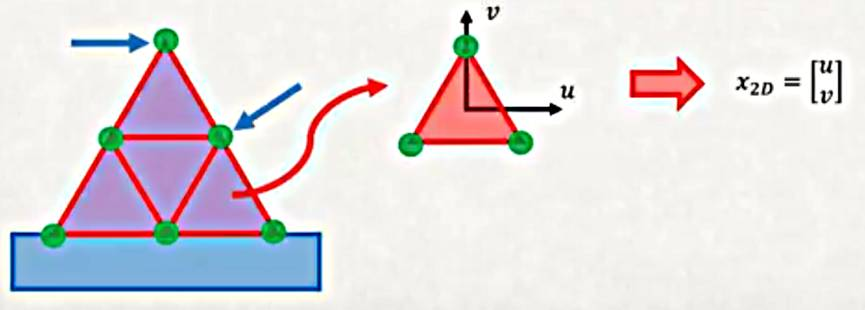
\includegraphics[width=20em]{compscieng_bpp45fem3_03.jpg}

Demek ki $x_{2D}$ vektörünü yaklaşıklamam lazım, genel bir metot şöyle olabilir,

$$
x_{2D} = \left[\begin{array}{c}
a_0 + a_1 X_1 + a_2 X_2 + a_3 X_1 X_2 + ...\\
b_0 + b_1 X_1 + b_2 X_2 + b_3 X_1 X_2 + ...
\end{array}\right]
$$

Tek yaptığımız tek yönde yaklaşıklama yerine iki yönde yaklaşık bir temsil
kullanmak. 

Fakat daha önce baktığımız 1D FEM örneğinden hatırlarsak yer değişim yaklaşık
fonksiyonunu düğümsel yer değişiklikleri ($u_i$ ve $v_i$) ve şekil fonksiyonları
($N_i$ gibi) üzerinden temsil etmek istiyoruz. Üstteki değişim tüm üçgene
bakıyor, biz üçgenin düğümlerini temsil etmek istiyoruz. 

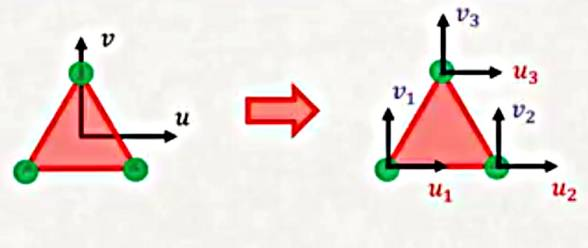
\includegraphics[width=20em]{compscieng_bpp45fem3_04.jpg}

O zaman herhangi bir FEM öğesi için yer değişimini, genel olarak, düğümleri
üzerinden

$$
x_{2D} = \left[\begin{array}{c}
u_1 N_1 + u_2 N_2 + .. + u_n N_N \\
v_1 N_1 + v_2 N_2 + .. + v_n N_N
\end{array}\right]
$$

ile gösterebilirim. Üstteki üçgen öğe örneğinde 

$$
x_{2D} = \left[\begin{array}{c}
u_1 N_1 + u_2 N_2 + u_3 N_3 \\
v_1 N_1 + v_2 N_2 + v_3 N_3
\end{array}\right]
$$

yeterlidir. $x_{2D}$ vektörünü bir matris vektör çarpımı haline getirebiliriz,

$$
x_{2D} = \left[\begin{array}{ccccccc}
N_1 & 0 & N_2 & 0 & \dots & N_n & 0 \\
0 & N_1 & 0 & N_2 & 0 & \dots & N_n 
\end{array}\right]
\left[\begin{array}{c}
u_1 \\ v_1 \\ u_2 \\ v_2 \\ \dots \\ u_n \\ v_n
\end{array}\right]
$$

Daha kisa olarak

$$
\implies x_{2D} = [N] u_e
$$

denebilir. Dikkat edersek $N$ fonksiyonları $X_1,X_2$ değişkenlerinin
birer fonksiyonu, $u_i,v_i$ değerleri ise sabit.

Bu noktada elimde genel bir yer degisim fonksiyonu var, onu kullanarak bir
gerilme (strain) vektoru hesaplayabilirim. Iki boyutta $\epsilon$'un sadece uc
tane ogesi var,

$$
\epsilon = \left[\begin{array}{c}
\epsilon_{11} \\ \epsilon_{22} \\ 2 \epsilon_{12} 
\end{array}\right]
$$



















[devam edecek]

Kaynaklar

[1] Petitt, {\em Intro to the Finite Element Method}, University of Alberta,
    \url{https://www.youtube.com/watch?v=2iUnfPRk6Ro&list=PLLSzlda_AXa3yQEJAb5JcmsVDy9i9K_fi}

[2] Petitt, {\em Finite Element Method Theory}, University of Alberta,
    \url{https://www.youtube.com/watch?v=2iUnfPRk6Ro&list=PLLSzlda_AXa3yQEJAb5JcmsVDy9i9K_fi}

[3] Bayramli, {\em Fizik, Materyel Mekanigi 2}
    
\end{document}
